\section{Systems}
\subsection{Design of the CSharp-MiniTwit application} \label{Design of the CSharp-MiniTwit application}
We have decided to convert the given source code into an application called 'Csharp-Minitwit' written in C\#. We have chosen C\# for its well documented ecosystem and robustness, due to it being statically and strongly typed, and we have chosen to build our app using the NET 8.0 runtime, as it is the latest long-term supported release (end of support Nov. 2026)\cite{netcoresupport}.

The application is built using the ASP.NET Core framework\cite{aspnetcoreintro2023}, with razor pages for rendering HTML pages, and we are following a Model-View-Controller (MVC) pattern and dependency injection, for easier maintainability and testability.\newline
The application itself requires a database for storing users, messages, followers and metadata. For this we have chosen to connect to a PostgreSQL using Entity Framework Core (an ORM), making subsequent database alterations and migrations easy.\newline


\todo{INSERT PICTURE - NOT WORKING RIGHT NOW}
\begin{figure}[ht]
    \centering
    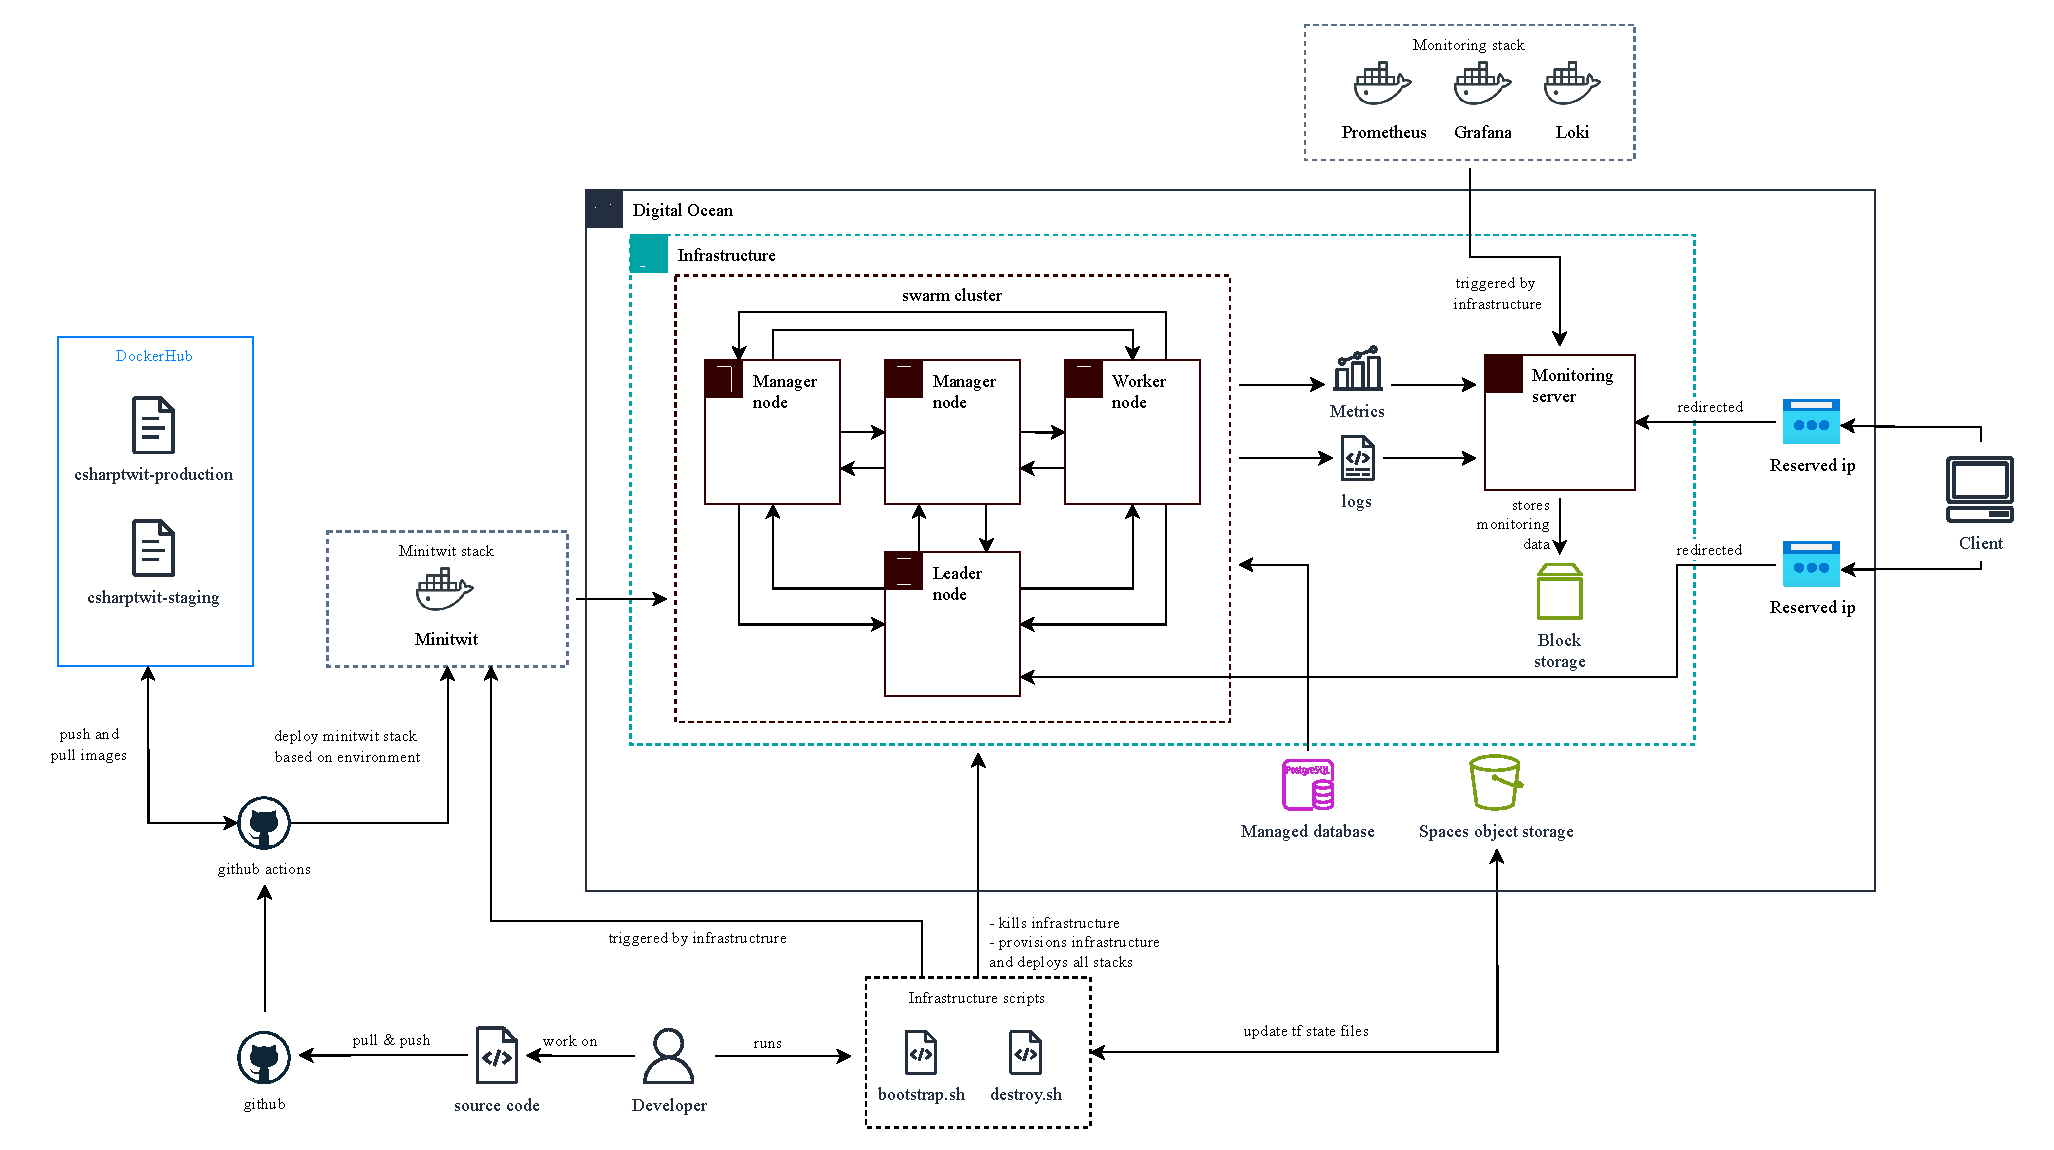
\includegraphics[height=0.8\textwidth, angle=90]{images/figures/devops-architecture-architecture_v2.pdf}
    \caption{System Architecture Diagram}
    \label{fig:architecture}
\end{figure}

Below we will zoom in on some of the important aspects of the system. 

\subsubsection{Versioning and CI/CD}
The application is versioned, tested, quality assured and deployed using
GitHub. Our group has been following the Gitflow workflow to avoid merge conflicts, and ensure tractability. Gitflow also allows us to have a 'develop' and a 'main' branch, enabling us to easily set up a staging server, for integration testing.\newline 
Our GitHub repository is also used for project management, creating issues and documentation. Deploying our application to our servers is done using GitHub actions, creating Docker images and pushing them to the relevant environment. GitHub actions also runs unit tests, formats our source code using 'dotnet format' and analyzes it using SonarCloud and Code Climate.\\\\
GitLab would have been a good alternative, however the whole group already have GitHub accounts and use it for personal projects — GitLab supports all the same features but is known for having a stronger focus on DevOps and CI/CD\cite{gitlabvsgithub}. GitLab allows for free self-hosting. 

\subsubsection{Cloud provider}
We have chosen DigitalOcean as our cloud provider, running our application on provisioned virtual machines that we manage our selves. DigitalOcean has been chosen for the sole reason that they offered \$200 in credits for students — enough for the entire project.\newline 
Since we are not using managed application services, pretty much any cloud provider would suit our needs. Had we gone with managed services, Azure would have been a good alternative due to its integrations for ASP.Net.

\subsubsection{Provisioning}
For provisioning we use Terraform, which has been chosen specifically for it being declarative. The Terraform scripts are run using the 'bootstrap.sh' script, which takes a single parameter; 'production' or 'staging'. This in turn provisions our entire system (except the database) and pushes the corresponding docker image to the Docker Swarm.

\subsubsection{Database}
As mentioned, the application uses a PostgreSQL database. We have opted to go with a managed database, for simplicity and to delegate reliability issues to DigitalOcean. A single vertically scaled database will be able to handle many concurrent users. If we needed to scale up substantiably, we would likely have to switch to a specialized distributed database system like Kafka, which the real X uses\cite{kafka}.

\subsubsection*{Monitoring and logging}
We use Prometheus in a pull-based configuration for business monitoring. This was implemented as part of the exercises and has been kept for that reason. We also use DigitalOcean's website for infrastructure monitoring, displaying CPU, memory and disk usage. We have no alarms / emails set up.\\\\
For logging we use Loki, which is inspired by Prometheus and chosen for that same reason\cite{Loki}.\\\\
Grafana is used to display Prometheus data as a dashboard, and to query the logs from Loki.

\subsubsection{Containerization and container orchestration}
The application is built as a Docker image through the CI/CD chain. From there it is deployed to an instance of Docker Swarm, using a compose file that connects our application with a Prometheus container. This setup has 2 replicas running on the swarm \todo{We have 2 replicas running across 5 VMs, why not have more?}\\
The Grafana server is setup using standard Grafana, Prometheus and Loki images, composed together in a \texttt{docker-compose.yml}.\\\\
The Docker Swarm is setup with 1 leader node, 2 manager nodes and 1 worker node. We only have a single worker node, as we have hit a max number of VMs, and we want to have both a staging and a production environment. To enable the leader node to crash and its role be taken by another node, it is required to have 2 manager nodes.\\\\

% Developers work on the source code, and merging the new features into the main branch trigger a deployment workflow that updates the application's Docker images on Dockerhub. A later step uploads the Terraform state files for infrastructure management, which pulls the updated images and initiates the infrastructure update process, deploying changes to Digital Ocean.

% Refer to \ref{apendix:systems-architecture} for a system's architecture diagram.

% \subsection{Important interactions of subsystems}
% \subsubsection{Docker Swarm - Csharp-Minitwit application}
% When deploying a Docker Swarm cluster, a reserved IP is assigned to the manager node. Users will use this IP to send requests to the Csharp-Minitwit application. When receiving a request, the Docker Swarm cluster routes it through its routing mesh to one of the worker nodes running an instance of the Csharp-Minitwit application, which will process the request and serve a response.

% \subsubsection{Serilog - Loki - Grafana}
% Serilog configures a C\# API that will receive the Csharp-Minitwit application logs and send them in a POST request to Loki's server. The structured representation of these Logs makes it easier to extract information from them at a later point. Loki can then be configured as a data source in Grafana to process and store these logs to be queried from a Dashboard.

% \subsubsection{Csharp-Minitwit - Prometheus - Grafana}
% When the Csharp-Minitwit application processes a request that executes one of the metrics methods, the OpenTelemetry.Exporter.Prometheus.AspNetCore package will collect and expose them on a \textit{/metrics} endpoint that will be scrapped by a Prometheus server at a given rate. Prometheus can then be used as a data source in Grafana, allowing us to feed a dashboard with this information. 
\subsection{Infrastructure}
\subsubsection{Application Dependencies}
% probably this info can be presented in tables with three columns (dev, staging, prod) and "X" pointing to the environment in which each is used.
Dependencies are handled using dotnet's package manager, NuGet:
\begin{itemize}
    \item Npgsql.EntityFrameworkCore.PostgreSQL 
    \item OpenTelemetry.Exporter.Prometheus.AspNetCore (exports telemetry data to Prometheus)
    \item OpenTelemetry.Extensions.Hosting
    \item Microsoft.EntityFrameworkCore (ORM)
    \item Serilog (structured logging library)
    \item Swashbuckle.AspNetCore (auto-generated Swagger documentation)
\end{itemize}

\subsubsection{Technologies used}
A quick overview of the technologies used:
\begin{itemize}
    \item \textbf{GitHub}: Code repository, versioning and project management.
    \item \textbf{SonarCloud}: ensuring quality in the code.
    \item \textbf{Digital Ocean}: hosting of virtual servers, databases and volumes.
    \item \textbf{Terraform}: provisioning and management of infrastructure on Digital Ocean.
    \item \textbf{Docker}: containerization of the application for deployment.
    \item \textbf{Prometheus}: monitoring system and time series database that collects metrics.
    \item \textbf{Loki}: log aggregation system integrated with Grafana for viewing logs.
    \item \textbf{Grafana}: visualization of metrics and logs.
\end{itemize} \todo{put in same order as subsubsections below}

\subsection{Interactions of subsystems}
\subsubsection{APIController/HomeController - ORM - Database} 
Incoming requests to the application are handled by either the \texttt{APIController} or the \texttt{HomeController}. Both provide similar endpoint logic but are meant to be used by the simulator and regular users respectively. A request's path will match a specific endpoint, prompting the application to perform a corresponding database operation. For instance a POST request to \textit{/login} will invoke the \texttt{GetByUsername} method from the \texttt{userRepository} and request the user information through an SQL SELECT query. The ORM will map the results back to C\# objects, which the controller returns in the HTTP response to the user.

Refer to Figure 4 in \ref{apendix:systems-architecture} for a sequence diagram showing how a user successfully follow another user and gets a response from the system. See Figure 5 in \ref{apendix:systems-architecture} for a sequence diagram illustrating how a request from the simulator is handled in the system.

\subsection{Current state of the systems}
% Current state of your systems, for example using results of static analysis and quality assessment systems.
% Double check that for all the weekly tasks (those in the end of the lecture notes) you include the corresponding information.
% MSc students remember to argue for the choice of technologies and decisions for at least all cases for which we asked you to do so in the tasks at the end of each session.